\documentclass[aspectratio=169,10pt]{beamer}
\usetheme{default}
\usecolortheme{default}
\setbeamertemplate{navigation symbols}{}
\setbeamertemplate{footline}[frame number]
\usepackage{booktabs}
\usepackage{pgfplots}
\pgfplotsset{compat=1.18}
\definecolor{accent}{RGB}{31,94,168}
\definecolor{quiet}{RGB}{150,150,150}
\setbeamercolor{frametitle}{fg=accent}
\setbeamercolor{title}{fg=accent}
\setbeamercolor{itemize item}{fg=accent}

\title{TF24 gradients in plant}
\subtitle{What the solver and controller work buys}
\date{8 October 2026}

\begin{document}

\begin{frame}
  \titlepage
\end{frame}

\begin{frame}{A TF24 gradient run costs 0.24--0.43 of brute force}
  \begin{columns}[T]
    \begin{column}{0.55\textwidth}
      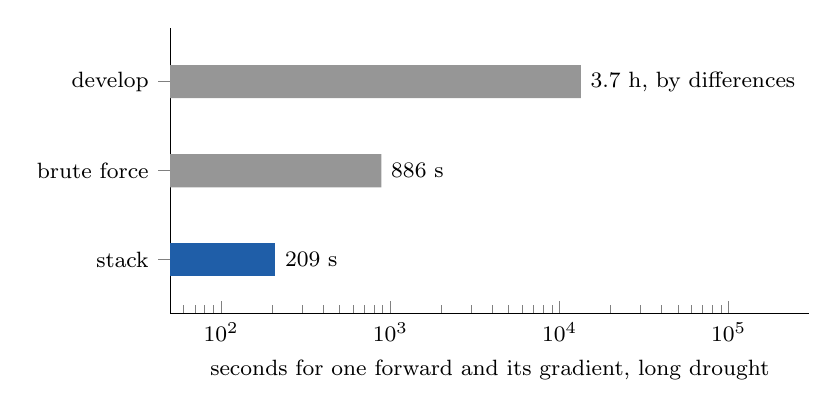
\begin{tikzpicture}
        \begin{axis}[xbar, width=0.8\linewidth, height=5.2cm, xmode=log, log basis x=10,
            xmin=50, xmax=300000, xlabel={seconds for one forward and its gradient, long drought},
            symbolic y coords={stack, brute force, develop}, ytick={stack, brute force, develop},
            nodes near coords, nodes near coords align={horizontal},
            every node near coord/.append style={font=\footnotesize, anchor=west},
            point meta=explicit symbolic, bar width=12pt, bar shift=0pt, enlarge y limits=0.3,
            axis x line*=bottom, axis y line*=left, every axis label/.style={font=\footnotesize},
            ticklabel style={font=\footnotesize}]
          \addplot[fill=quiet, draw=none] coordinates
            {(13354,develop) [3.7 h, by differences] (886,brute force) [886 s]};
          \addplot[fill=accent, draw=none] coordinates {(209,stack) [209 s]};
        \end{axis}
      \end{tikzpicture}
    \end{column}
    \begin{column}{0.4\textwidth}
      \small
      \begin{itemize}
        \item \textbf{0.24} of brute force at 108 nodes, the pilot included; episodic within 0.40$\varepsilon$ of it.
        \item \textbf{0.43} at 215 nodes, which long drought needs to match brute force's accuracy.
        \item \texttt{develop} has no gradient: 100 forwards by central differences.
        \item Nothing fails across five rainfall records.
      \end{itemize}
    \end{column}
  \end{columns}
  \vfill
  {\scriptsize\color{quiet} Timed alone, one run each. \texttt{docs/measurements/headline/}}
\end{frame}

\begin{frame}{Why: what an evolutionary analysis needs from TF24}
  \begin{itemize}
    \item One singular strategy: \textbf{about 84 runs}: resident forwards, invader walks, reverse sweeps.
    \item Each answer within $\varepsilon$ of converged: 0.025 in $\ln J$, a tenth of each elasticity's spread over eight weather seeds.
  \end{itemize}
  \bigskip
  Before this work:
  \begin{itemize}
    \item \textbf{No gradients}: about 98 forwards each, by differences.
    \item \textbf{Walks failed} on episodic and dry rain: 27--38-day steps, pools stable for 26.
    \item \textbf{Error went unreported}: companions saw 0.33--0.41 of the node error.
    \item \textbf{Gradients were staircases} at sign changes; curvatures off by up to 13$\varepsilon$.
  \end{itemize}
\end{frame}

\begin{frame}{What changed: four groups, 17 branches, every default off}
  \small
  \begin{tabular}{@{}p{0.2\textwidth}p{0.75\textwidth}@{}}
    \toprule
    \textbf{Gradients} & exact counts; the reverse sweep; exact invader replay; the first invasion walks the recording \\
    \textbf{The split} & per-state error weights; a node's step split where its net production changes sign, forward and in the sweep \\
    \textbf{Settings} & \texttt{control\_tf24()}: tied tolerance, soil weight, bound, 15-day cap; the soil stepped alone; \texttt{control\_window()} from a pilot \\
    \textbf{Node rule} & crowns sorted; the spread (D); walks by birth date \\
    \bottomrule
  \end{tabular}
  \bigskip

  On the aornugent forks, one issue each. The stack sits on odelia 0.5.0 and needs a rebase onto upstream \texttt{develop} (odelia 0.6.2).
\end{frame}

\begin{frame}{The reverse sweep: every gradient for 2.5 forwards}
  \begin{itemize}
    \item One sweep costs \textbf{2.5--2.7 forwards} at any node count.
    \item Matches central differences to 7e-4 of the resident's \texttt{lma} elasticity.
    \item Replaces about 98 forwards of differences per gradient.
    \item Invaders replay the resident's recorded steps: at the resident's traits $J' = J$ to the bit.
  \end{itemize}
\end{frame}

\begin{frame}{The split: gradients without staircases}
  \begin{itemize}
    \item Where a cohort's net production changes sign inside a step, its step is cut there.
    \item $\ln J$ lies \textbf{3--13$\times$ nearer} the converged answer wherever nodes cross.
    \item A $\pm5\%$ tolerance nudge moves no gradient entry past $\varepsilon/6$; up to 0.52$\varepsilon$ without.
    \item The sweep through it is within 2e-3 of central differences on every record.
    \item Cost: +5--9\% of a gradient run.
  \end{itemize}
\end{frame}

\begin{frame}{Settings: spend accuracy where fitness is earned}
  \begin{itemize}
    \item \texttt{control\_tf24()} names TF24's setting once; with the window it saves \textbf{31--34\%} of a gradient run.
    \item The \textbf{15-day cap} removes the episodic and dry walk failures.
    \item The \textbf{soil stepped alone} where the stand draws little water: a gradient run takes 0.63 of the time, every elasticity within 0.063$\varepsilon$.
    \item The \textbf{window}: tolerance loosened once most of $J$ is earned, read off a cheap pilot. On five records nothing fails, $\ln J$ within 5.8e-5 of a 1e-6 reference.
  \end{itemize}
\end{frame}

\begin{frame}{The node rule: an error that reports itself}
  \begin{itemize}
    \item \textbf{The spread}: each birth-date interval's leaf area spread over point crowns.
    \item Uniform nodes converge at the square law: ratios 3.5--4.0 on long-wet and dry.
    \item A half-node companion reports \textbf{0.87--0.99} of the error, against 0.33--0.41 before.
    \item Cost: +6.7\% of a gradient run with splits on.
    \item Walks by birth date: a shared thinned schedule saves 24--25\% of a walk, selection gradient within 0.004$\varepsilon$.
  \end{itemize}
\end{frame}

\begin{frame}{Accuracy against brute force, and where nodes matter}
  \centering\small
  \begin{tabular}{@{}lrrr@{}}
    \toprule
    against the two-rung answer, long drought & median & largest & time vs brute force \\
    \midrule
    brute force, 215 nodes, 1e-5 & 0.12$\varepsilon$ & 0.49$\varepsilon$ & 1 \\
    the stack, 215 nodes & 0.13$\varepsilon$ & 0.53$\varepsilon$ & 0.43 \\
    the stack, 108 nodes & 0.50$\varepsilon$ & 2.1$\varepsilon$ & 0.24 \\
    \bottomrule
  \end{tabular}
  \bigskip
  \begin{itemize}
    \item On episodic the stack at 108 nodes is within 0.40$\varepsilon$ of brute force on all 50 entries.
    \item On long drought 108 nodes are too few; the companion run is what tells you so.
  \end{itemize}
\end{frame}

\begin{frame}{What moves for existing users}
  \begin{itemize}
    \item Every new behaviour is off by default and bit-identical when off.
    \item The \textbf{height coordinate}, plant's default, does not move.
    \item \textbf{FF16 on the birth-date coordinate} moves: the deep-crown anchor 17.14 $\to$ 18.01. Its error at the default schedule is larger, but falls at the square law, so it can be estimated.
    \item TF24 model versions v11--v13.
    \item Under default \texttt{Control()}, TF24's $J$ on long drought is 0.45 against 12.75 converged: the defaults, not the model, carry the gap.
  \end{itemize}
\end{frame}

\begin{frame}{Open, and how to review}
  \begin{columns}[T]
    \begin{column}{0.48\textwidth}
      \textbf{Open}
      \begin{itemize}\small
        \item Episodic needs nodes finer than its dry spells (past 429).
        \item The constant record's later nodes move its gradients up to 3$\varepsilon$.
        \item Diagnostics next: each run's error estimate, distance from the grid, failures.
        \item The radius one grid serves is unmeasured.
      \end{itemize}
    \end{column}
    \begin{column}{0.48\textwidth}
      \textbf{Review in four PR groups}
      \begin{enumerate}\small
        \item Gradients (\texttt{PLANT-93}--\texttt{99})
        \item The split (\texttt{PLANT-100}--\texttt{103}, odelia\#53--54)
        \item Settings (\texttt{PLANT-104}--\texttt{106}, odelia\#55)
        \item Node rule (\texttt{PLANT-107}--\texttt{109}): the FF16 question
      \end{enumerate}
    \end{column}
  \end{columns}
\end{frame}

\end{document}
